% This is "sig-alternate.tex" V1.9 April 2009
% This file should be compiled with V2.4 of "sig-alternate.cls" April 2009
%
% This example file demonstrates the use of the 'sig-alternate.cls'
% V2.4 LaTeX2e document class file. It is for those submitting
% articles to ACM Conference Proceedings WHO DO NOT WISH TO
% STRICTLY ADHERE TO THE SIGS (PUBS-BOARD-ENDORSED) STYLE.
% The 'sig-alternate.cls' file will produce a similar-looking,
% albeit, 'tighter' paper resulting in, invariably, fewer pages.
%
% ----------------------------------------------------------------------------------------------------------------
% This .tex file (and associated .cls V2.4) produces:
% 1) The Permission Statement
% 2) The Conference (location) Info information
% 3) The Copyright Line with ACM data
% 4) NO page numbers
%
% as against the acm_proc_article-sp.cls file which
% DOES NOT produce 1) thru' 3) above.
%
% Using 'sig-alternate.cls' you have control, however, from within
% the source .tex file, over both the CopyrightYear
% (defaulted to 200X) and the ACM Copyright Data
% (defaulted to X-XXXXX-XX-X/XX/XX).
% e.g.
% \CopyrightYear{2007} will cause 2007 to appear in the copyright line.
% \crdata{0-12345-67-8/90/12} will cause 0-12345-67-8/90/12 to appear in the copyright line.
%
% ---------------------------------------------------------------------------------------------------------------
% This .tex source is an example which *does* use
% the .bib file (from which the .bbl file % is produced).
% REMEMBER HOWEVER: After having produced the .bbl file,
% and prior to final submission, you *NEED* to 'insert'
% your .bbl file into your source .tex file so as to provide
% ONE 'self-contained' source file.
%
% ================= IF YOU HAVE QUESTIONS =======================
% Questions regarding the SIGS styles, SIGS policies and
% procedures, Conferences etc. should be sent to
% Adrienne Griscti (griscti@acm.org)
%
% Technical questions _only_ to
% Gerald Murray (murray@hq.acm.org)
% ===============================================================
%
% For tracking purposes - this is V1.9 - April 2009
\documentclass{sig-alternate}
% Import some more mathematical symbols

\usepackage{graphicx}
\usepackage{makeidx}
\usepackage{verbatim}

\usepackage{latexsym}
% Use eps figures
\usepackage{epsfig}
% Different array macros, e.g. table row height modification
\usepackage{subfigure}
\usepackage{array}
% Import some more mathematical symbols
\usepackage{amsmath,amssymb,mathtools}
% Import an algorithm formatting package
%\usepackage[vlined,algoruled,titlenumbered]{algorithm2e}
% Use an extension of the verbatim package
\usepackage{url}
%\usepackage[colorlinks=true]{hyperref}

% Define some theorems
\newtheorem{lemma}{Lemma}[section]
\newtheorem{theorem}[lemma]{Theorem}
\newtheorem{hypothesis}[lemma]{Hypothesis}

% Define other symbols
\newcommand{\R}{\mathbb{R}}
\def\argmax{\operatornamewithlimits{arg\max}}
\def\argmin{\operatornamewithlimits{arg\min}}
\def\supmax{\operatornamewithlimits{arg\sup}}
\newcommand{\grad}{\nabla}
\newcommand{\I}{\mathbb{I}}
\newcommand{\Fro}{\mathrm{Fro}}
\newcommand{\Obj}{\mathit{Obj}}
\newcommand{\pcbf}{\mathit{pcbf}}
\newcommand{\pmcf}{\mathit{pmcf}}
\newcommand{\phy}{\mathit{phy}}
\newcommand{\ru}{\mathit{ru}}
\newcommand{\rv}{\mathit{rv}}
\newcommand{\rw}{\mathit{rw}}
\newcommand{\rs}{\mathit{rs}}
\newcommand{\rss}{\mathit{rss}}
\newcommand{\rsc}{\mathit{rsc}}
\newcommand{\rscs}{\mathit{rscs}}
\newcommand{\tr}{\operatorname{tr}}
\newcommand{\diag}{\operatorname{diag}}
\renewcommand{\a}{\vec{a}}
\renewcommand{\b}{\vec{b}}
\renewcommand{\c}{\vec{c}}
\newcommand{\x}{\vec{x}}
\newcommand{\y}{\vec{y}}
\newcommand{\z}{\vec{z}}
\newcommand{\w}{\vec{w}}
\newcommand{\f}{\vec{f}}
\renewcommand{\r}{\vec{r}}
\newcommand{\s}{\vec{s}}
\renewcommand{\t}{\vec{t}}
\renewcommand{\L}{\mathcal{L}}
\newcommand{\la}{\langle}
\newcommand{\ra}{\rangle}
\renewcommand{\vec}[1]{\mathbf{#1}}

% Define a fourth level subheading (Scott)
\newcommand{\subfour}{\vspace*{3mm}\hspace{-2.5mm}}
\newcommand{\subfive}{\hspace{2.5mm}}

% Define a command for extended commenting (Scott)
\long\def\COMMENT#1\ENDCOMMENT{\message{(Commented text...)}\par}

\begin{document}
%
% --- Author Metadata here ---
\conferenceinfo{WWW}{'12 Lyon, France}
%\CopyrightYear{2007} % Allows default copyright year (200X) to be over-ridden - IF NEED BE.
%\crdata{0-12345-67-8/90/01} % Allows default copyright data (0-89791-88-6/97/05) to be over-ridden - IF NEED BE.
% --- End of Author Metadata ---
\title{New Objective Functions for Social Collaborative Filtering}
%\titlenote{(Produces the permission block, and
%copyright information). For use with
%SIG-ALTERNATE.CLS. Supported by ACM.}

\numberofauthors{7} % in this sample file, there are a *total*
% of EIGHT authors. SIX appear on the 'first-page' (for formatting
% reasons) and the remaining two appear in the \additionalauthors section.
%
% Joseph, Scott, Nguyen, Peter, Lexing, Edwin, Ehsan
\author{
\alignauthor
Joseph Noel\\
\affaddr{ANU}\\
\affaddr{Canberra, Australia}\\
\email{jinonoel@gmail.com}
\alignauthor
Scott Sanner\\
\affaddr{NICTA \& ANU}\\
\affaddr{Canberra, Australia}\\
\email{first.last@nicta.com.au}
\alignauthor
Khoi-Nguyen Tran\\
\affaddr{ANU}\\
\affaddr{Canberra, Australia}\\
\email{first.last@anu.edu.au}
\and
\alignauthor
Peter Christen\\
\affaddr{ANU}\\
\affaddr{Canberra, Australia}\\
\email{first.last@anu.edu.au}
\alignauthor
Lexing Xie\\
\affaddr{ANU}\\
\affaddr{Canberra, Australia}\\
\email{first.last@anu.edu.au}
\alignauthor
Edwin Bonilla\\
\affaddr{NICTA \& ANU}\\
\affaddr{Canberra, Australia}\\
\email{first.last@nicta.com.au}
}
\additionalauthors{
Additional authors: Ehsan Abbasnejad (ANU \& NICTA,
email: {\texttt{first.last@nicta.com.au}}).}
%\author{
%\alignauthor
%Anonymous\\
%\affaddr{Unknown}\\
%}
\maketitle
\begin{abstract}
This paper examines the problem of social \emph{collaborative
filtering} (CF) algorithms to recommend items of interest to users in
a social network setting.  Unlike standard CF algorithms using
relatively simple user and item features, recommendation in social
networks poses the more complex problem of learning user preferences
from a rich and complex set of user profile and interaction
information.  Many existing \emph{social CF} methods have extended
% NOTE: Separating out information diffusion and social regularization
% aspects may be important for revising this paper in future.
traditional CF \emph{matrix factorization}, but have overlooked
important aspects germane to the social setting; specifically,
existing matrix factorization methods (a) do not exploit user features
in all aspects of learning, (b) do not permit directly modeling
user-to-user information diffusion, and (c) use objectives that treat
users as globally (dis)similar even though they may only be
(dis)similar in specific latent areas of interest.  This paper
proposes a unified framework for social CF matrix factorization that
addresses (a)--(c) by introducing novel objective functions for
training.  We demonstrate that optimizing these new objectives
significantly outperforms a variety of CF and social CF baselines on
live user trials in a custom-developed Facebook App involving data
collected over two months from over 100 App users and their 34,000+
friends.
\end{abstract}
\category{H.3.3}{Information Search and Retrieval}{information filtering}
\terms{Algorithms, Experimentation}
\keywords{social networks, collaborative filtering, machine learning}

\section{Introduction}
\label{sec:Introduction}
%!TEX root = document.tex

\label{sec:introduction}

% motivate socical recommendation 
Online social networks such as Facebook record a rich set of user
preferences (likes of links, posts, photos, videos), user traits,
interactions and activities (conversation streams, tagging, group
memberships, interests, personal history and demographic data).  This
presents myriad new dimensions to the recommendation problem by making
available a rich labeled graph structure of social interactions and
content from which user preferences can be learned and new
recommendations can be made.

Existing recommendation methods for social networks aggregate this
rich social information into a simple measure of user-to-user interaction 
that can be leveraged to model user homophily via social
regularization~\cite{lla,socinf,sr,rrmf, Noel2012NOF}, a trust
ensemble~\cite{ste}, or a low-rank factorization of the social
interactions matrix~\cite{sorec}.  But in aggregating all of these
interactions and common activities into a single strength of
interaction, we 
%show effectively that the signal present in this 
%information gets drowned out in the noise --- some fine-grained
%interactions and activities are highly informative, but most are not.
ask whether important preference information has been discarded?
Indeed, the point of departure for this work is the hypothesis that
different fine-grained interactions (e.g. commenting on a wall or
getting tagged in a video) and activities (e.g., being a member of a
university alumni group or a fan of a TV series) \emph{do} represent
different preferential {\em affinities} between users, and moreover
that effective {\em filtering} of this information (i.e., learning
which of these fine-grained interactions and activities are 
informative) will lead to improved accuracy in social recommendation.

%% No longer fits cleanly in the intro, should be moved into related
%% work is not already mentioned there.  -SPS
\eat{
In the context of recent work on social
recommendation~\cite{sorec,ste,lla} and information diffusion
~\cite{Goel2012structure,Romero2011hashtag,Bakshy2012chamber}, it is
important to know which of these interactions or common traits are
actually reflective of common preferences.}

To quantitatively validate our hypotheses and evaluate the
informativeness of different fine-grained features for social
recommendation, we have built a Facebook App to collect detailed user
interaction and activity history available through the Facebook Graph
API along with user preferences solicited by the App on a daily basis.
Specifically, each day our App recommends three links to each App user
that are collected from the timeline of other users (both friends and
non-friends) and we record users' explicit likes and dislikes of these
recommended links.  Given this data, we define \emph{social affinity
groups (SAGs)} of a target user (ego) as sets of surrogate users
(alters) serving as proxies for an ego's preferences; these SAGs are
defined according to fine-grained
\emph{interactions} (e.g., users who have been tagged in the target user's
video) and \emph{activities} (e.g., users who have liked the same
political party page that the target user has liked).  Given a set of
SAGS for a user, (1) we define a novel recommendation method called
{\em social affinity filtering (SAF)} where we learn to predict
whether a user will like an item based on the surrogate item
preferences of members of each SAG, and (2) we analyse the relative
informativeness of SAGs across a variety of dimensions such as type,
frequency of friend preferences, and activity membership size.

In the four months that our App was active, we collected data for a
set of Facebook app users and their full interactions with 38,000+
friends along with 22 distinct types of interaction and users activity
for 3000+ groups, 4000+ favourites, and 10,000+ pages.  In subsequent
sections that outline our experimental methodology and results in
detail, we make the following critical observations:
\begin{itemize}
\item We found that SAF significantly 
outperforms numerous state-of-the-art collaborative filtering and social recommender 
systems, by up to 6\% in accuracy using just \emph{page} (like) features.
Because the reluctance of a user to install an App increases with the number
of permissions requested, this suggests a state-of-the-art social recommendation App 
need only request permissions for a user's \emph{page} likes in order to achieve
state-of-the-art recommendation accuracy.
% -- in short, these fine-grained features can be very informative.
% Also, what about combining all features?  Not enough data?  -SPS
% Probably also much faster -- should we show a table of train and test times?  -SPS
\item We found that groups, pages, and favourites make for more informative
SAGs than those defined by user-to-user interactions.  This is likely because the former can be
applied to SAGs over the entire Facebook population 
rather than just a user's friends (where the data is considerably limited).
\item Among the interactions, we found that those on videos are more predictive than those on other content types (photos, post, link), and that outgoing interactions (performed by the ego on the alter's timeline) 
are more predictive than incoming ones (performed by alters on the
ego's timeline), although the level of exposure of an ego to an
alter's preferences is more important than the directionality of the
interaction with the alters.
% Below: not sure I quite understand ``persistent'' and ``temporally synchronized'' here... 
% are there better terms or can they be further (briefly) explained?  -SPS
\item %{\bf TODO: see Latex comments.} 
Among {\em groups}, {\em pages} and {\em favourites}, we found that only
a small subset of the features were actually informative, bringing into question the efficacy of 
previous social recommendation approaches that aggregate social information between
two users into a single numerical value.  We found that the most  
predictive activity SAGs tend to have small memberships.  We also found features
corresponding to ``long-tailed'' content (such as music and books)
can be much more predictive than those with fewer choices 
(e.g. interests or sports). 
 %to generic (such as interests) or activities that require 
 %simultaneous participation (such as sports) are less predictive of 
 %user interest than topics that are ongoing or persistent in time (such as TV, books).
\end{itemize}
As detailed in the subsequent sections, these findings not only
demonstrate the power of leveraging fine-grained interaction and
activity features but they also suggest which of these features can
be most informative when building state-of-the-art
SAF-based recommenders.
%  This
%latter point is quite important since as already noted, there is
%a trade-off between the number of permissions a Facebook App requests
%and user uptake.
%
%we note later -- the more
%permissions an App requests, the less likely a user is to grant
%permissions to the App, so choosing permissions (i.e., social
%features) well is crucial for achieving good recommendations with
%minimal intrusion into a user's privacy.

\eat{
To better understand these subtleties and to understand what
social interactions and user traits reflect common preferences on
Facebook, we proceed in the following sections to describe our data,
our experimental methodology, and various analyses according to our
methodology that shed light on the above questions. 
On one hand our observations confirm certain observations made previous 
on different networks, such as the diminishing returns of repeated exposures, 
on the other we also see a few new clues such as 
that very specific types of outgoing interactions are more predictive 
than other interactions. 
We then conclude with a summary of the key novel observations arising
from this study.
}

\yum



\section{Definitions and Background}
\label{sec:Background}
%%
%% Template intro.tex
%%

\chapter{Background}
\label{cha:back}

In the following section, we define the source of our data set, notation used throughout this thesis, our choice of classification algorithms and 
our testing approach and methodology.

\section{Facebook}
\label{sec:data}

Facebook is the largest and most active social media service in the world. Facebook users can create a profile containing personal 
preferences and information (age, birthday, group preferences, favourite athlete, etc) and have friendships and interactions 
between other users. The four main interactions between users are posts (posting an element on a friends' wall), tags
(being mentioned in a friends post or comment), comments (written data on a post) and likes (clicking a like button if a user 
likes a post or comment). The three mediums for these interactions are across links (some URL), posts (some Facebook post), 
photos (some uploaded Facebook photo) and videos (some uploaded Facebook video).

\begin{figure}[h]
	\begin{center}
		\includegraphics[scale=0.85]{results/imageLiked.png}
		\caption{Here we see an example of a link posted to a friends wall, which has subsequently been liked by two friends.}
	\end{center}
\end{figure}

\clearpage
One issue present in this Facebook paradigm is discovering whether a user doesn't like an item, a users Facebook feed is comprised of 
activity between their friends, content, groups, etc given the enormous scope of potential feed items, Facebook will only show feed 
items for users who you have recently interacted with using their \emph{Edge-Rank} ~\cite{edge} algorithm. 

While many Facebook users have a friend count which is close to the human real word limit, known as the Dunbar number 
~\cite{hill2003social}, the \emph{Edge-Rank} algorithm ensures user interactions are focused on a much smaller subset of their friends.
Additionally, given the rate of posting, these top feed items are only displayed for a short amount of time. This is coupled 
with the fact that Facebook allows users to explicitly like an item, but not dislike it - hence distinguishing between what 
a user does and does not like becomes difficult.

Given this issue, NICTA have developed an app which explicitly determines a users preference for an item, by facilitating explicit 
like and dislike options, which will be discussed in the following section.

%\cite{backstrom2011center} studied two types of user uses of Facebook, explicit communication interaction and viewing attention. Communication 
%is focused on a limited subset of friends whilst viewing attention is dispersed among a much larger set. This supports the approach of testing
%a wide array of user interactiuons and preferences, as each users preferences are driven by where their attention is focused.

\section{LinkR}
\label{sec:linkr}

NICTA developed a Facebook app named \emph{LinkR} \footnote{The main developer of the LinkR Facebook App is Khoi-Nguyen Tran, 
a PhD student at the Australian National University.} which would make recommendations to users and record whether or not the 
user liked the recommended item.

The app also collected information about users, their interactions and preferences as well as a subset of available information about 
their friends. The app tracked and stored information for over 100 app users and their 39,000+ friends over a 4-month time period.

The table below summarises the data collected from both app users and their friends.

\begin{table}[!htbp]
\centering
	\begin{tabular}{|l|r|r|r|r|} % cols: (left, center, right)
		\hline
		\textbf{App Users} & \textbf{Posts} & \textbf{Tags} & \textbf{Comments} & \textbf{Likes}  \\ \hline
		\textbf{Wall} & 27,955 & 5,256 & 15,121 & 11,033 \\ \hline
		\textbf{Link} & 3,974 & - & 5,757 & 4,279 \\ \hline
		\textbf{Photo} & 4,147 & 22,633 & 8,677 & 5,938 \\ \hline
		\textbf{Video} & 211 & 2,105 & 1,687 & 710 \\ \hline
		 \hline
		\textbf{App Users and Friends} & \textbf{Posts} & \textbf{Tags} & \textbf{Comments} & \textbf{Likes}  \\ \hline
		\textbf{Wall} & 3,384,740 & 912,687 & 2,152,321 & 1,555,225 \\ \hline
		\textbf{Link} & 514,475 & - & 693,930 & 666,631 \\ \hline
		\textbf{Photo} & 1,098,679 & 8,407,822 & 2,978,635 & 1,960,138 \\ \hline
		\textbf{Video} & 56,241 & 858,054 & 463,401 & 308,763 \\ \hline
	\end{tabular}
	\caption{Data records for interactions between users. Rows are the type of interaction, columns are the medium.}
	\label{tab:revpol}
\end{table}

\clearpage

Pertinent user features we will exploit during this thesis include:
\begin{itemize}
\item Gender
\item Age
\item Hometown
\item Locale
\item Group Memberships
\item Page Likes
\item Favourite Activities
\item Favourite Books
\item Favourite Athletes
\item Favourite Teams
\item Inspirational People
\item Interests
\item Favourite Movies
\item Favourite Music
\item Favourite Sports
\item Favourite Television Shows
\item School Information
\item Work Information
\item Messages data
\end{itemize}

\section{Notation}
\label{sec:notation}

The mathematical notation used by our classifiers during this thesis are outlined below.

\begin{itemize}
\item A set of users of size $N$. 
\item A set of items of size $M$.
\item A user feature vector $X$ of size $i$, the size of each feature vector varies based on the current user features being analysed
and is explicitly defined in each section. In other words $X = \langle x_1, x_2, \dots , x_i \rangle$
\item A set of alters $A$ of size $j$, the size and composition of each alters set varied based on the current user features being 
analysed and is explicitly defined in each section.
\item An exposure of size $k$, where each $k$ represents the number of some user $n$'s friends who have liked some item $m$.
\item A data-set $D$ comprised of $D = \{(n,m,x_i) \to y\}$ with the binary response $y \in \{0,1\}$ where $0$ represents a dislike 
and $1$ represents a like.
\end{itemize}

\section{Feature Vectors}
\label{sec:features}

Individual feature vectors for $X$ will be discussed and defined in their appropriate sections under \emph{User Interactions} and 
\emph{User Preferences}. During this thesis we will analyse the results gained from the $7$ different user features listed below, 
additionally a combination of the most predictive individual feature vectors will also be tested.

\begin{itemize}
\item Interactions
\item Demographics
\item Traits
\item Groups
\item Pages
\item Outgoing Messages
\item Incoming Messages
\end{itemize}

\section{Previous Work}
\label{sec:pw}

Below we discuss previous work done in this classification area completed in 2011 by Joseph Noel.

\subsection{Social Collaborative Filtering}
\label{sec:cbf}

Two general approaches to classification prediction are \emph{content-based filtering} (CBF) ~\cite{newsweeder} which exploits 
item features based on items a user has previously liked, or the second approach which is \emph{collaborative filtering} (CF) 
~\cite{collab_filtering} which exploits the current user's preferences as well as those of other users.

Previous work defined the term \emph{social} CF (SCF) ~\cite{joseph} which augments traditional CF methods with additional social 
network information, the results of this previous work and analysis came to the conclusion that the approach of \emph{Social Matchbox}
provided the best results for this data set. In live user trials SMB provided the best performance against all other implemented 
algorithms and as such will be used as a baseline in this thesis.

\section{Training and Testing}
\label{sec:tt}

All evaluation is done using 10 fold cross validation wherein the data is partitioned into 10 complimentary subsets, each 
subset is composed of two separate parts, one part is used for training $(80\%)$ and the other $(20\%)$ is used for testing. 
All training and testing is performed on each distinct fold and the results are averaged along with their standard error in each
table and graph.

\section{Classification Algorithms}
\label{sec:meth}

Each classification algorithm used in this thesis is passed the training set for each fold as discussed previously. Based on this 
data and the current feature vector $X$ the classifier builds a model representation of the data and uses this model to classify 
each component in the test set into either a like or a dislike.

All feature vector analysis carried out in this thesis will be performed on the following classification algorithms.

\subsection{Constant}
\label{sec:const}

The constant (Constant) predictor returns a constant result irrespective of the feature vectors selected. The most common result 
in our data set is $False$ and hence the $False$ predictor is displayed in all analysis, tables and graphs.

\subsection{Social Match Box}
\label{sec:sr}

SMB is an extension of existing SCF techniques~\cite{lla,socinf} which constrain the latent space to enforce users 
who have similar preferences to maintain similar latent representations when they interact heavily.

SMB uses the \emph{Social Regularization} method which incorporates user features to learn
similarities between users in the latent space which allows us to incorporate the social information of the Facebook data ~\cite{joseph}.
This objective component constrains users with a high similarity rating to have the same values in the latent feature space, which
models the assumption that users who are similar socially should also have similar preferences for items.

\subsection{Naive Bayes}
\label{sec:nb}

\emph{Naive Bayes} is a basic probabilistic classifier which involves applying Bayes' theorem using strong conditional independence 
assumptions between each feature in $X$. During training each element $i$ in the feature vector is devised to contribute some 
evidence that this $X$ belongs to either a like or dislike classification, during testing the class with the highest probability 
when applied to the model is the classification returned. 

The NB implementation used during this thesis is an implementation previously devised by Scott Sanner.
\footnote{Scott Sanner is a Senior Researcher in the Machine Learning Group at NICTA and the supervisor for this research.}.

\subsection{Logistic Regression}
\label{sec:lr}

\emph{Logistic Regression} directly estimates parameters based on the training data assuming a parametric form of the distribution.
LR predicts the odds of a feature vector $X$ being either a like or a dislike by converting a dependent variable and 
one or more continuous independent variable(s) into probability odds.

The LR implementation used during this thesis is \emph{LingPipe} \cite{lin}.

\subsection{Support Vector Machine}
\label{sec:svm}

The \emph{Support Vector Machine} is a supervised learning machine based on a set of basis functions which help construct 
a separating hyperplane between data points. Training involves building the relevant hyperplanes which can then be used for testing. 
Each data point is classified as a like or dislike depending on which side of the hyperplane it falls.

The SVM implementation used during this thesis is \emph{SVMLibLinear} \cite{cjlin}.

\section{Evaluation Metrics}
\label{sec:notation}

When evaluating the success of each feature vector at correctly classifying an item, the following metrics will be analysed.

\begin{itemize}
\item A \emph{true positive} (TP) prediction refers to when the classifier correctly identifies the class as true. 
\item A \emph{false positive} (FP) occurs when the prediction is true, but the true class was false. 
\item A \emph{false negative} (FN) occurs when the prediction is false but the actual class is true.
\end{itemize}

Accuracy relates to the closeness to the true value. In the context of our results, the accuracy refers to the number of correct classifications 
divided by the size of the data set.

\[ \text{accuracy} = \frac{\text{number of correct classifications}}{\text{size of the test data set}}\]

Precision relates to the number of retrieved predictions which are relevant. In the context of our results, the precision refers to the number of TP predictions 
divided by the sum of the TP and FP predictions.

\[ \text{precision} = \frac{\text{number of TP}}{\text{number of TP + number of FP}}\]

Recall refers to the number of relevant predictions that are retrieved. In the context of our results, recall refers to the number of TP predictions 
divided by the sum of the TP and FN predictions.

\[ \text{recall} = \frac{\text{number of TP}}{\text{number of TP + number of FN}}\]

The f-score combines and balances both precision and recall and is interpreted as the weighted average of both precision and recall. 

\[ \text{f-score} = 2 \times \frac{\text{precision} \times \text{recall}}{\text{precision} + \text{recall}}\]

The main metric we use for analysis, tabulation and graphing in this thesis is accuracy.

%%% Local Variables: 
%%% mode: latex
%%% TeX-master: "thesis"
%%% End: 


\section{New Objective Functions for SCF}
\label{sec:NewObjFuns}
Having surveyed previous CF work, especially MF-based CF and SCF
methods, we now present the major conceptual contributions of the
paper.  We begin by introducing a unified
matrix factorization framework for optimizing all MF objectives
evaluated in this paper --- old and new.
%, including newly proposed objectives to
%address observed deficiencies of SCF MF methods as outlined in
%Section~\ref{sec:Introduction}.

\subsection{A Composable Objective Framework}

%\subsubsection{Composable Objectives}

We take a composable approach to MF-based (S)CF, where an optimization
objective $\mathit{Obj}$ is composed of sums of one or more objective
components:
\begin{align}
\mathit{Obj} = \sum_i \lambda_i \mathit{Obj}_i
\end{align}
Because each objective may be weighted differently, a weighting term
$\lambda_i \in \R$ is included for each component.  In the current
work, we manually tuned each $\lambda_i$, except for the \emph{first} 
$i$ in $\sum_i$, which can be set as $\lambda_i = 1$ without loss of
generality.

Most target predictions in this paper are binary ($\{0,1\}$),
therefore a sigmoidal transform $\sigma(o) = \frac{1}{1 + e^{-o}}$ of
a prediction $o \in \R$ may be used to squash it to the range $[0,
1]$.  Where the $\sigma$ transform may be optionally
included, this is written as $[\sigma]$.  While $\sigma$ transforms
are generally advocated for real-valued regressor outputs when used in
a classification setting, we note that our experiments showed little
variation in results whether including or omitting it, although
including it tended to slow the convergence of gradient optimization.
Nonetheless, where appropriate, we include the possibility of a
$\sigma$ transform since it may prove useful in other settings.

\subsection{Existing Objective Functions}

For completeness, we first cover a number of known objective
components that are used in the objectives evaluated and
extended in this paper.  A discussion of gradient optimization along
with all necessary derivatives for these objectives is provided in
Appendix~\ref{app:Derivatives}.

\subsubsection{Matchbox-style Matrix Factorization ($\Obj_\pmcf$)}

\label{sec:matchbox_def}

%As a first step towards addressing our first observed deficiency that
%%the six surveyed SCF MF methods of Section~\ref{sec:scf_original} do not
%exploit user or item features.  In extending these methods to support
%features, we must first identify
In Section~\ref{sec:mf}, we discussed an MF objective~\eqref{eq:basic_mf}
that \emph{did not} make use of user or item features.  
However, if we \emph{do} have user feature vector $\x$ 
and item feature vector $\y$, we can respectively
represent the latent projections of user and item as $(U \x)_{1 \ldots
K}$ and $(V \y)_{1 \ldots K}$ and hence use $\la U \x, V \y \ra = \x^T
U^T V \y$ as a measure of affinity between user $\x$ and item $\y$.
Substituting the feature-based $\x^T U^T V \y$ for the featureless 
$U_\x^T V_\y$ in~\eqref{eq:basic_mf}, we arrive at the form of the basic CF 
objective function used in \emph{Matchbox}~\cite{matchbox} --- although
Matchbox used Bayesian optimization methods, we can easily express
its main objective in the following log likelihood form:
\begin{align}
\Obj_\pmcf & = \sum_{(\x,\y) \in D} \frac{1}{2} (R_{\x,\y} - [\sigma] \x^T U^T V \y)^2 \label{eq:matchbox_obj}
\end{align}
%It should be clear that if $\x$ and $\y$ are simply binary vectors
%of mutually exclusive user and item IDs, then this form reduces
%to~\eqref{eq:basic_mf}.  However, in general it permits general real-valued
%feature vectors for $\x$ and $\y$ and hence a feature-based MF approach to CF.

\subsubsection{Regularization of $U$, $V$ \& $\w$ ($\Obj_\ru, \Obj_\rv, \Obj_\w$)}
%
To help in generalization, it is important to regularize any free
matrix parameters $U$ and $V$ (e.g., from
Section~\ref{sec:matchbox_def}) or vector parameters $\w$ (e.g., from
Section~\ref{sec:cbf}) to prevent overfitting  
% in the presence of
when dealing with 
sparse data. This can be done with a simple $L_2$ regularizer that
models a spherical Gaussian prior % of $0$  % ebonilla
on the parameters.  This
regularization component can be specified for $U$, $V$, and $\w$ 
% simply % ebonilla
 as follows:
\begin{align}
\Obj_\ru & = \frac{1}{2} \| U \|_\Fro^2 = \frac{1}{2} \tr(U^T U) \qquad
\Obj_\rv = \frac{1}{2} \tr(V^T V) \nonumber \\
\Obj_\rw & = \frac{1}{2} \| \w \|_2^2 = \frac{1}{2} \w^T \w \label{eq:reg}
\end{align}

\subsection{New Objective Functions}

\label{sec:newobjfun_defs}

Now we return to our observations concerning the deficiencies of
existing SCF MF methods as outlined in Section~\ref{sec:Introduction}
and propose new objective functions to address these issues.
Gradient-based optimization for these new objectives and all necessary
derivatives are covered in Appendix~\ref{app:Derivatives}.

\subsubsection{Feature Social Regularization ($\Obj_\rs$ \& $\Obj_\rss$)}
\label{sec:SocRec}

Our previous discussion of SCF methods in Section~\ref{sec:scf_original}
covered three different methods for \emph{social regularization} --- that is,
constraining users to be similar based on evidence from the social network.
However, none of these previous three SCF social regularization methods
exploited user features in the \emph{learning} process; more precisely 
$U_\x$ and $U_\z$ were regularized, but not the feature-based latent
spaces $U\x$ and $U\z$.  Hence if a gender difference in $\x$ and $\z$ was the
crucial factor to differentiating the latent spaces of each user, this could 
be \emph{learned} if we had a way of socially regularizing $U\x$ and $U\z$
directly.  To address this, we provide two variants of 
\emph{feature-based social regularization}.

The first new objective is an extension of simple 
\emph{social regularization}~\cite{lla,socinf} by incorporating user
features into that objective:
\begin{align}
\Obj_\rs = & \sum_{\x} \sum_{\z \in \mathit{friends}(\x)} \frac{1}{2} (S_{\x,\z} - \la U\x, U\z \ra)^2 \\
& = \sum_{\x} \sum_{\z \in \mathit{friends}(\x)} \frac{1}{2} (S_{\x,\z} - \x^T U^T U \z)^2 \nonumber 
\end{align}

%\subsubsection{Social Spectral Regularization ($\Obj_\rss$)}

Alternately, we could extend \emph{social spectral
regularization}~\cite{sr,rrmf} by incorporating user features into its
objective:
\begin{align}
\Obj_\rss = & \sum_{\x} \sum_{\z \in \mathit{friends}(\x)} \frac{1}{2} S^+_{\x,\z} \| U\x - U\z \|_2^2 \\
%& = \sum_{\x} \sum_{\z \in \mathit{friends}(\x)} \frac{1}{2} S^+_{\x,\z} \| U (\x - \z) \|_2^2 \nonumber \\
& = \sum_{\x} \sum_{\z \in \mathit{friends}(\x)} \frac{1}{2} S^+_{\x,\z} (\x - \z)^T U^T U (\x - \z) \nonumber
\end{align}

While we note these extensions are straightforward, they have the
simple property that they allow the system to learn the latent user
projection matrix $U$ \emph{as a function of user features} in order
to minimize the social regularization penalty.  Just as the Matchbox
objective in Section~\ref{sec:matchbox_def} allows us to exploit user
and item features in MF-based CF, these new social regularization
objectives permit more flexibility in exploiting user features in
\emph{learning} user similarity.
%Compared to non-socially regularized CF objectives, we will
%demonstrate that both of these approaches are quite powerful in 
%Section~\ref{sec:EmpResults}.

%\subfive Note: standard spectral regularization 
%assumes $S^+_{\x,\z} \in [0,1]$;
%however we may also want to try $S_{\x,\z}$ since a negative value
%actively encourages the latent spaces to oppose each other, which may
%be desired.

\subsubsection{Hybrid Information Diffusion + SCF ($\Obj_\phy$ )}

\label{sec:hybrid_scf}

One major weakness of MF methods is that they cannot model direct
joint features over user and items --- they must model user and item
features independently in order to compute the independent latent
projections $U\x$ and $U\z$.  Unfortunately, this prevents standard MF
objectives from modeling direct user-to-user information
diffusion~\cite{inf_diffusion} --- the unidirectional flow of
information (e.g., links) from one user to another.  This is
problematic because if user $\x$ \emph{always} likes what $\z$ has
posted or liked, then we would like to shortcut the latent
representation and simply learn to recommend user $\z$'s liked or 
posted items to user $\x$.

We fix this deficiency of MF by introducing another objective component
in addition to the standard MF objective, which serves as
a simple linear regressor for such information diffusion
observations.  The resulting hybrid objective component then becomes a
combination of latent MF and linear regression objectives.

For the linear regressor $\w^T \f_{\x,\y}$, we make use of the
\emph{same} weight vector $\w$ and feature vector $\f_{\x,\y}$
mentioned in Section~\ref{sec:cbf}; $\f_{\x,\y}$ is fully defined for
our empirical evaluation in Section~\ref{sec:fxy_def}.  As previously
noted, $\f_{\x,\y}$ includes
\emph{joint} user and item features from the social network, in
particular binary
\emph{information diffusion}~\cite{inf_diffusion} features
for \emph{each} friend $\z \in \mathit{friends}_\x$ indicating if $\z$
liked (or disliked) $\y$.  As a consequence, learning $\w$ allows the
linear regressor to predict in a personalized way for any user $\x$
whether they are likely to follow their friend $\z$'s preference for $\y$.

Formally, to define our hybrid information diffusion plus SCF objective,
we additively combine the output of the linear regression prediction with the
Matchbox prediction:
\begin{align}
\sqm \Obj_\phy = \sum_{(\x,\y) \in D} \frac{1}{2} (R_{\x,\y} - [\sigma] \w^T \f_{\x,\y} - [\sigma] \x^T U^T V y)^2 
\end{align}
%While again we note that this simple hybrid MF plus linear regression
%objective is straightforward, the ability to use joint user and item
%features to model information diffusion between users turns out to be 
%extremely powerful in our later experiments.

\subsubsection{Co-preference Regularization ($\Obj_\rsc$)}
\label{sec:rsc}

A crucial aspect missing from other SCF methods is that while two
users may not be globally similar or opposite in their preferences,
there may be sub-areas of their interests which can be correlated to
each other.  For example, two friends may have similar interests
concerning technology news, but different interests concerning
political news.  \emph{Co-preference regularization} aims to learn
such selective co-preferences.  The motivation is to constrain users
$\x$ and $\z$ who have similar or opposing preferences to be similar
or opposite in the \emph{same} latent item space relevant to item $\y$.

We use $\la \cdot, \cdot \ra_{\bullet}$ to denote a re-weighted inner
product. The purpose of this inner product is to ``mask'' enforcement
of latent space similarities or dissimilarities between users to be restricted
to the same latent spaces as the co-preferred items.  To this end, the
objective component for \emph{co-preference regularization} 
along with its expanded form is
\begin{align}
\Obj_\rsc & = \sum_{(\x,\z,\y) \in C} \frac{1}{2} (P_{\x,\z,\y} - \la U\x, U\z \ra_{V\y})^2 \\
& = \sum_{(\x,\z,\y) \in C} \frac{1}{2} (P_{\x,\z,\y} - \x^T U^T \diag(V\y) U \z)^2 \nonumber
\end{align}
We might also define a \emph{social co-preference spectral
regularization} approach, but our experiments so far have not indicated
this works as well as the above objective.  

In contrast to social regularization
defined previously, co-preference regularization does not require knowledge
of friendships or user interactions to determine co-preferences and hence
can enforce regularization constraints between \emph{all} users.
%can 
%can find correlations between users who are not friends --- this important
%observation will indeed surface in our forthcoming experimental evaluation.

\begin{comment}
\subsubsection{Social Co-preference Spectral Regularization ($\Obj_\rscs$)}
This is the same as the social co-preference regularization above, except that it uses the spectral regularizer format for 
learning the co-preferences.

 We use $\| \cdot \|_{2,\bullet}$ to denote a re-weighted $L_2$ norm. The reweighing of this norm servers the same purpose as the re-weighted inner product in Section~\ref{sec:rsc}, it tailors the similarities or dissimilarities between users to specific sets of items. This allows users $\x$
and $\z$ to be similar or opposite in the same latent latent space
relevant only to item $\y$.  
 
 The objective component for
 social co-preference spectral regularization along with its expanded form is
 
\begin{align}
\Obj_\rscs & = \sum_{(\x,\z,\y) \in C} \frac{1}{2} P_{\x,\z,\y} \| U\x - U\z \|_{2,V\y}^2 \\
%& = \sum_{(\x,\z,\y) \in C} \frac{1}{2} P_{\x,\z,\y} \| U (\x - \z) \|_{2,V\y}^2 \nonumber \\
& = \sum_{(\x,\z,\y) \in C} \frac{1}{2} P_{\x,\z,\y} (\x - \z)^T U^T \diag(V\y) U (\x - \z) \nonumber 
\end{align}
\end{comment}


\section{Evaluation Methodology}
\label{sec:Evaluation}
In this chapter we first discuss our Facebook Link Recommendation
(LinkR) application, specific definitions for user and item features
as well as definitions of an interaction, and our evaluation
methodology.

\subsection{Link Recommendation App on Facebook}

To evaluate existing and newly proposed CF and SCF methods discussed in
this paper, we created a Facebook application (i.e., a Facebook
``App'') that recommends links to users everyday, where the users may
give their feedback on the links indicating whether they \emph{liked}
it or \emph{disliked} it.  Figure~\ref{fig:linkr_app} shows a portion
of the Facebook LinkR App as it appears to users.

%%%%%%%%%%%%%%%%%%%%%%%%%%%%%%%%%%%%%%%%%%%%%%%%%%%%%%%%%%%%%%%%%%%%
\begin{figure}[t!]
\hspace{-2mm} \subfigure{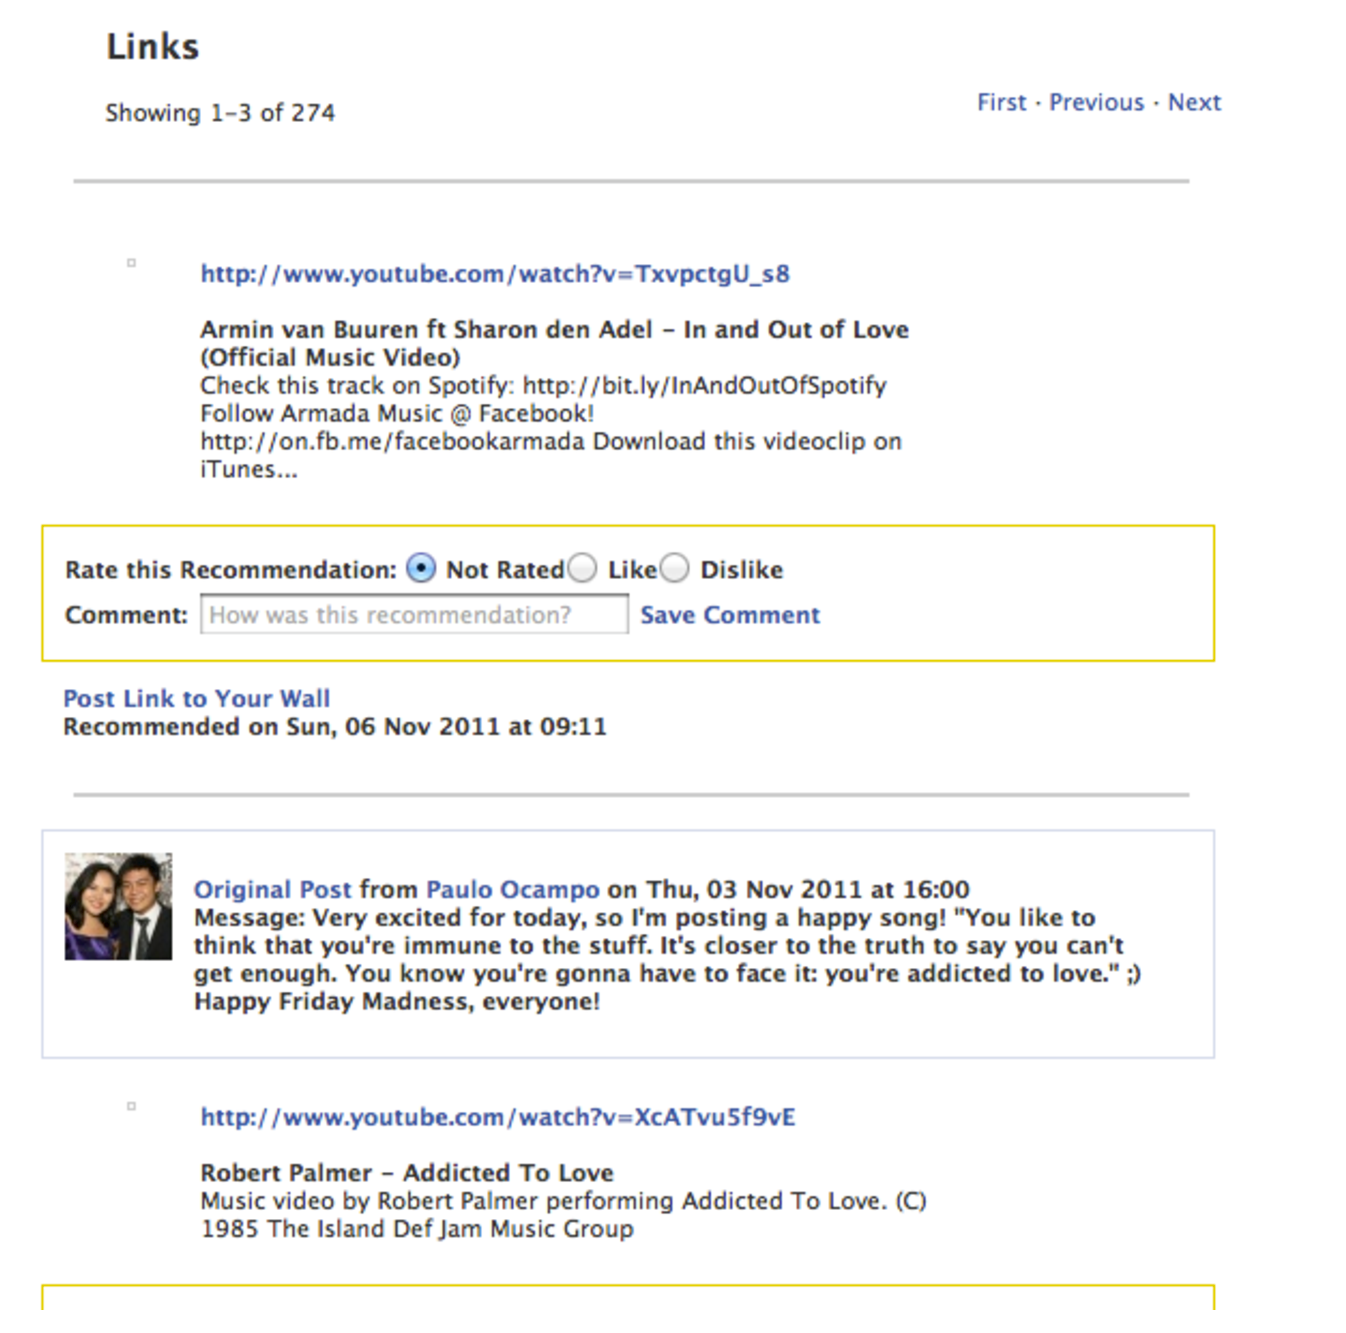
\includegraphics[scale=0.42]{img/linkr.eps}}
\caption{The Facebook LinkR App showing two link recommendations to a 
user.  One link recommendation is from a friend and includes the
friend's commentary on the link as well as the generic link
description extracted from meta-tags at the link source.  The other link
recommendation is from a non-friend and hence only shows the link
description extracted from meta-tags at the link source.
Users have the option of liking or disliking a recommendation
as well as providing explicit feedback commentary.}
\label{fig:linkr_app}
\end{figure}
%%%%%%%%%%%%%%%%%%%%%%%%%%%%%%%%%%%%%%%%%%%%%%%%%%%%%%%%%%%%%%%%%%%%

We discuss this application in detail next.

\subsubsection{LinkR}

Facebook allows applications to be developed that can be installed by
their users.  As part of this thesis project, the LinkR Facebook
application was developed.  The functionalities of the LinkR application
are as follows:
\begin{enumerate}
\item{Collect data that have been shared by users and their friends on Facebook.}
\item{Recommend (three) links to the users daily.}
\item{Collect feedback from the users on whether they liked or disliked the recommendations.}
\end{enumerate}



\subsection{Dataset}

\label{sec:dataset}

Using the LinkR Facebook App developed for this project, we were able
to gather data on 34,860 users and 437,023 links.

\subsubsection{User Data}

Date that are collected and used for the user features are as follows:
\begin{itemize}
\item {Gender:} male or female
\item {Birthday:} year
\item {$\mathit{location}_\mathit{id}$:} an integer ID corresponding
to the user's specific present location (city and country)
\item {$\mathit{hometown}_\mathit{id}$:} an integer ID corresponding
to the user's specific home town (city and country)
\item {$F_{\x,\z} \in \{ 0, 1\}$:} indicator of whether 
users $\x$ and $\z$ are friends.
% Joseph: be specific here...
\item {$\mathit{Int}_{\x,\z} \in \mathbb{N}$:} interactions on
Facebook between users $\x$ and $\z$ as defined in Section~\ref{sec:notation}.
\end{itemize}

\subsubsection{Link Data}

Data that are used for the link features are:
\begin{itemize}
\item{$\mathit{id}$ of the user who posted the link.}
\item{$\mathit{id}$ of the user on whose wall the link was posted.}
\item{Text description of the link from the user who posted it.}
\item{Text link summary from the metatags on the target link webpage.}
\item{Number of times the link has been liked.}
\item{Number of times the link has been shared.}
\item{Number of comments posted on the link}.
\item {$F'_{\x,\y} \in \{0, 1\}$:} indicator of whether user $\x$ has liked item $\y$.
\end{itemize}
Additionally, links that have been recommended by the LinkR
application have the following extra features:
\begin{itemize}
\item{$\mathit{id}$'s of users who have clicked on the link url.}
\item{Optional ``Like'' or ``Dislike'' rating of the LinkR user on the link.}
\end{itemize}

\subsubsection{Interaction Data}
\label{sec:interactions}

The interactions between users that we count (equally weighted) to define
$\mathit{Int}_{\x,\z}$ are:

\begin{enumerate}
\item{Being friends.}
\item{Posting an item (link, photo, video, photo, or message) on a user's wall.}
\item{Liking an item (link, photo, video, photo, or message) on a user's wall.}
\item{Commenting on an item (link, photo, video, photo, or message) on a user's wall.}
\item{Being tagged together in the same photo.}
\item{Being tagged together in the same video.}
\item{Two users tagging themselves as attending the same school.}
\item{Two users tagging themselves as attending the same class in school.}
\item{Two users tagging themselves as playing sports together.}
\item{Two users tagging themselves as working together for the same company.}
\item{Two users tagging themselves as working together on the same project for the same company.}
\end{enumerate}

\subsubsection{Live Online Recommendation Trials}

For the recommendations made to the LinkR application users, we select
only links posted in the most recent two weeks that the user has not
liked. We use only the links from the last two weeks since an informal
user study has indicated a preference for recent links.  Furthermore,
older links have a greater chance of being outdated and are also
likely to represent broken links that are not working anymore. We have
settled on recommending three links per day to the LinkR users and
according to the survey done at the end of the first trial, three
links per day seems to be the generally preferred number of
daily recommendations.

For the live trials, Facebook users who installed the LinkR
application were \emph{randomly assigned one of four algorithms in
each of the two trials}. Users were not informed which algorithm was
assigned to them to remove any bias. We distinguish our recommended
links into two major classes, links that were posted by the LinkR
user's friends and links that were posted by users other than the
LinkR user's friends. The LinkR users were encouraged to rate the
links that were recommended to them, and even provide feedback
comments on the specific links. In turn these ratings became part of
the training data for the recommendation algorithms, and thus were used
to improve the performance of the algorithms over time. Based on the
user feedback, we filtered out non-English links and links without any
descriptions from the recommendations to prevent user annoyance.

At the end of the first trial, we conducted a user survey with the
LinkR users to find out how satisfied they were with the
recommendations they were getting.
 

\section{Baseline Comparision}
\label{sec:Baselines}
In this chapter we discuss the first set of four SCF algorithms that
was implemented for the LinkR application and then show how each
algorithm performed during the live user trial, how satisfied the
users were with links being recommended to them through LinkR, and the
results of offline passive experiments with the algorithms.

\subsection{Algorithms}

The CF and SCF algorithms used for the first user trial were:

\begin{enumerate}
\item{ {\bf $k$-Nearest Neighbor (KNN)}: We use the user-based approach as described in Section~\ref{sec:nn}.}
\item{{\bf Support Vector Machines (SVM)}: We use the the SVM implementation described in Section~\ref{sec:svm} using the features described in Section~\ref{sec:dataset}.}
\item{{\bf Matchbox (Mbox)}: Matchbox MF  + L2 $U$ Regularization + L2 $V$ Regularization}
\item{{\bf Social Matchbox (Soc. Mbox)}: Matchbox MF + Social Regularization + L2 Regularization}
\end{enumerate}

Social Matchbox uses the Social Regularization method to incorporate the social information of the FB data. SVM incorporates social information in the $\f_{\x,\y}$ features that it uses. Matchbox and Nearest Neighbors do not make use of any social information.

\subsection{Online Results}

The first live user trial was run from August 25 to October 13. The algorithms were randomly distributed among the 106 users who installed the LinkR application. The distribution of the algorithms to the users are show in Table~\ref{tab:Assigned1}

\begin{table}[t!]
\centering
\begin{tabular}{| l | c |}
\hline
{\bf Algorithm} & {\bf Users} \\
\hline
Social Matchbox & 26\\
Matchbox  & 26 \\
SVM & 28 \\
Nearest Neighbor & 28 \\
\hline
\end{tabular}
\caption{Number of Users Assigned per Algorithm.}
\label{tab:Assigned1}
\end{table}

Each user was recommended three links everyday and they were able to
rate the links on whether they `Liked' or `Disliked' it. Results shown
in Figure~\ref{fig:OnlineResult1} are the percentage of Like ratings
and the percentage of Dislike ratings per algorithm stacked on top of
each other with the Like ratings on top.

As shown in Figure~\ref{fig:OnlineResult1}, Social Matchbox was the
best performing algorithm in the first trial and in fact was the only
algorithm to get receive more like ratings than dislike ratings. This
would suggest that using social information does indeed provide useful
information that resulted in better link recommendations from LinkR.

\begin{figure*}[t!]
\centering
\subfigure{\includegraphics[scale=0.28]{img/live-likes1.eps}}
\subfigure{\includegraphics[scale=0.28]{img/live-friend-likes1.eps}}
\subfigure{\includegraphics[scale=0.28]{img/live-nonfriend-likes1.eps}}
%\subfigure{\includegraphics[scale=0.35]{img/live-dislikes1.eps}}
\caption{Results of the online live trials. The percentage of Liked
ratings are stacked on top of the percentage of Disliked ratings per
algorithm. Social Matchbox was found to be the best performing of the
four algorithms evaluated in the first trial.  *** Results of the online
live trials, split between friends and non-friends. The percentage of
Liked ratings are stacked on top of the percentage of Disliked ratings
per algorithm. There is a significant drop in performance between
recommending friend links and recommending non-friend links.}
\label{fig:OnlineResult1}
\end{figure*}

We also look at the algorithms with the results split between friend
links and non-friend links recommendations. Again, the results shown
in Figure~\ref{fig:OnlineFriend1} are the percentage of Like ratings
and the percentage of Dislike ratings per algorithm stacked on top of
each other with the Like ratings on top. As shown in
Figure~\ref{fig:OnlineFriend1}, all four algorithms experienced a
significant performance drop in the ratio of Likes to Dislikes when it
came to recommending non-friend links. This suggests that aside from
Liking or Disliking a link solely from the quality of the link being
recommended, users are also more likely to Like a link simply because
a friend had posted it and more likely to Dislike it because it was
posted by a stranger.

\subsection{Survey Results}

Near the end of the first trial, the LinkR users were invited to answer a survey regarding their experiences with the recommendations they were getting. They were asked a number of questions, with the following pertaining to the quality of the recommendations:

\begin{itemize}
\item{Do you find that ANU LinkR recommends interesting links that you may not have otherwise seen?}
\item{Do you feel that ANU LinkR has adapted to your preferences since you first started using it?}
\item{How relevant are the daily recommended links?}
\item{Overall, how satisfied are you with LinkR?}
\end{itemize}

They gave their answers to each question as an integer rating with range $[1-5]$, with a higher value being better. Results are shown in Figure~\ref{fig:survey1}. Their answers were grouped together according to the recommendation algorithm that was assigned to them, and the averages per algorithm are below.

As shown in Figure~\ref{fig:survey1}, Social Matchbox achieved higher survey scores than the other recommendation algorithms, in all four questions. The results of the survey reflected the results in the online live trial and confirms that Social Matchbox was the best recommendation algorithm in the first trial.
 
\begin{figure*}[t!]
\centering
\subfigure{\includegraphics[scale=0.23]{img/not-seen.eps}}
\hspace{-6mm} \subfigure{\includegraphics[scale=0.23]{img/relevant.eps}}
\hspace{-6mm} \subfigure{\includegraphics[scale=0.23]{img/adapted.eps}}
\hspace{-6mm} \subfigure{\includegraphics[scale=0.23]{img/satisfied.eps}}
\caption{Results of the user survey after the first trial. The survey answers from the users reflect the online results that Social Matchbox was the best recommendation algorithm in this trial.}
\label{fig:survey1}
\end{figure*}

\subsection{Summary}
At the end of the first trial, we have observed the following:

\begin{itemize}
\item{Social Matchbox was the best performing algorithm in the live user trial in terms of percentage of likes.}

\item{Social Matchbox received the highest user evaluation scores in the user survey at the end of the user trial.}

\item{Of the various combinations of training and testing data in the offline passive experiment, we found that training on the UNION subset and testing on the APP-USER-ACTIVE-ALL subset best correlated with the results of the live user trial and the user survey. Training on the UNION dataset had advantages compared to training on the other data subsets, namely that it had the large amount of information of the PASSIVE data and the explicit dislikes information of the ACTIVE data.}

\begin{comment}
Explain which offline evaluation correlates with both of these user feedback metrics... can you briefly explain why?  E.g., training on UNION gives you explicit negatives, which are crucial (side note, perhaps not for thesis: except maybe for NN which actually does need negatives!), and ranking evaluation really requires an accurate list of likes/dislikes for an accurate ranking metric which can only be had with the active data}
\end{comment}

\end{itemize}

In the next chapter, we discuss new techniques for incorporating social information and show how they improve on Social Matchbox.


\section{Novel Algorithms for Social Recommendation}
\label{sec:NovelAlgs}
\subsection{Second Trial}

For the second online trial, we chose four algorithms again to
randomly split between the LinkR application users. Social Matchbox
was included again as a baseline since it was the best performing
algorithm in the first trial. The distribution count of the algorithms
to the users is shown in Table~\ref{tab:assigned2}

The four SCF algorithms are:

\begin{itemize}
\item{{\bf Social Matchbox (Soc. Mbox)} : Matchbox MF + Social Regularization +  L2 $U$ Regularization + L2 $V$ Regularization}
\item{{\bf Spectral Matchbox (Spec. Mbox)}: Matchbox MF + Social Spectral Regularization + L2 $U$ Regularization + L2 $V$ Regularization}
\item{{\bf Social Hybrid (Soc. Hybrid)}: Hybrid + Social Regularization + L2 $U$ Regularization + L2 $V$ Regularization + L2 $\w$ Regularization}
\item{{\bf Spectral Co-preference (Spec. CP)}: Matchbox MF + Social Co-preference Spectral Regularization + L2 $U$ Regularization + L2 $V$ Regularization}
\end{itemize}

\subsubsection{Online Results}
\label{sec:online2}

The online experiments were switched to the new algorithms on October
13, 2011. For the online results reported here, since the second live
trial is still currently ongoing, we took a snapshot of the data as it
was on October 22, 2011. The algorithms were randomly distributed
among the 103 users who still had the LinkR application installed. The
distribution of the algorithms to the users are show in
Table~\ref{tab:assigned2}


\begin{table}[t!]
\centering
\begin{tabular}{| l | c |}
\hline
{\bf Algorithm} & {\bf Users} \\
\hline
Social Matchbox & 26\\
Spectral Matchbox  & 25 \\
Spectral Co-preference & 27 \\
Social Hybrid & 25 \\
\hline
\end{tabular}
\caption{Number of Users Assigned per Algorithm.}
\label{tab:assigned2}
\end{table}

Results shown in Figure~\ref{fig:online2} are the percentage of Like
ratings and the percentage of Dislike ratings per algorithm stacked on
top of each other with the Like ratings on top.

First thing we note in Figure~\ref{fig:online2} is the decrease in
performance for Social Matchbox, and in fact for all SCF algorithms in
general. Except for Spectral Matchbox, they all received more Dislike
ratings than Like ratings. What we noticed is that of the
recommendations being made in the week that we switched over to the
new algorithms, the majority of the links were about Steve Jobs, who
had died the week previously. We believe that the redundancy and lack
of variety of the links being recommended caused an increase in the
Dislike ratings being given by users on the recommended links. Taking
out the skewed results that follows an unusual event such as this, the
relative algorithm performance was better.

%%%%%%%%%%%%%%%%%%%%%%%%%%%%%%%%%%%%%%%%%%%%%%%%%%%%%%%%%%%%%%%%%%%%%%%%%
\begin{figure*}[t!]
\centering
\subfigure{\includegraphics[scale=0.28]{img/live-likes2.eps}}
\subfigure{\includegraphics[scale=0.28]{img/live-friend-likes2.eps}}
\subfigure{\includegraphics[scale=0.28]{img/live-nonfriend-likes2.eps}}
\caption{Results of online live trials. The percentage of Liked
ratings are stacked on top of the percentage of Disliked ratings per
algorithm. Spectral Matchbox achieved the highest ratio of likes to
dislikes among the four algorithms. Spectral social regularization in
general appears to be a better way to socially regularize compared to
social regularization. *** Results of the online live trials, split
between friends and non-friends. As in the first trial, there is a
significant drop in performance between recommending friend links and
recommending non-friend links.}
\label{fig:online2}
\end{figure*}
%%%%%%%%%%%%%%%%%%%%%%%%%%%%%%%%%%%%%%%%%%%%%%%%%%%%%%%%%%%%%%%%%%%%%%%%%

We again split the results again between friend link recommendations
and non-friend link recommendations, with the results shown in
Figure~\ref{fig:online2} being the percentage of Like ratings and the
percentage of Dislike ratings per algorithm stacked on top of each
other with the Like ratings on top.  As shown
Figure~\ref{fig:online2}, all four algorithms experienced significant
performance drop in the number of likes when it came to recommending
non-friend links. This reflects the results of the first trial.
 
\begin{comment}
Additionally, the differences were more drastic with the two
algorithms that uses the social regularization method: Social Matchbox
and Social Hybrid. This, together with results of the first user
trial, seems to confirm our earlier analysis that aside from Liking or
Disliking a link just from the quality of the links being recommended,
users are also more likely to like a link because a friend had posted
it and more likely to dislike it because it came from a stranger.
\end{comment}

We note the following observations from the results shown in Figures
\ref{fig:online2}:

\begin{itemize}
\item{Compared to the other algorithms, Spectral Matchbox achieved the
best ratio of likes to dislikes as seen, as seen in
Figure~\ref{fig:online2}. Combined with the results for Spectral
Co-preference, Spectral social regularization in general appears to be
a better way to socially regularize compared to social
regularization. This comparison holds even when the results are split
between friend links recommendations and non-friend links
recommendations, as seen in Figure~\ref{fig:online2}.}

\item{When looking at just the friend link recommendations in
Figure~\ref{fig:online2}, Social Hybrid was the best performing
algorithm. This result comes from the user-user information diffusion
among its friends that Social Hybrid learns, which could not be
learned by the other SCF algorithms. Learning information diffusion
thus helps when it comes to building better SCF algorithms.}

\item{Spectral Co-preference didn't do well on friend link
recommendations, however it did better on the non-friend link
recommendations. When it comes to recommending friend links, friend
interaction information coming through social regularizer seems more
important than implicit co-likes information provided by the
co-preference regularizer. When there is no social interaction
information such as with non-friend links, co-preference methods with
its implicit co-likes information appear much better than just vanilla
collaborative filtering at projecting users into subspaces of common
interest.}
\end{itemize}

\subsection{Summary}

We summarize the observations made during the second trial:

\begin{itemize}
\item{The social spectral regularization methods generally performed
better in the live user trials, even when the results were split
between friend link recommendations and non-friend link
recommendations.}

\item{Learning information diffusion models helps in SCF, as evidenced
by the strong performance of Social Hybrid when recommending friend
links.}

\item{When there is no social interaction information, learning
implicit co-likes information is better than using plain CF methods.}

\item{The better performance of the social spectral regularization
methods in the live trials were not reflected in the offline
experiments. Perhaps there is a better metric than MAP that correlates
with human preferences.}
\end{itemize}



\section{Conclusions}
\label{sec:Conclusions}
In concluding our evaluation in this paper, we 
confirmed many previous observations of related work: saturation
effects~\cite{Romero2011hashtag}, the importance of directionality of
interactions~\cite{saez2011high}, and the importance of real
vs. virtual interactions~\cite{brandtzag2011facebook}.  This work also
elucidated some fascinating new insights.  For one, 
saturation effects in exposure curves have been noted
by~\cite{Romero2011hashtag} to be topic-dependent --- in this work
we note that they are \emph{also} social 
\emph{interaction-dependent}.  Secondly, certain interactions are
highly predictive of certain \textit{Like Types} and certain specific
\emph{Interaction Directions}, \emph{Modalitities}, and \emph{Actions}
are far more predictive of general likes (i.e., outgoing photo likes)
than others.  Finally, common user traits such as \emph{Interests} and
\emph{History} display interesting and unusual trends w.r.t.\ exposure
and group size that indicate different social mechanisms may be at
work behind some of these traits --- an important topic for future
exploration.

Perhaps most importantly though, comparing the overall predictiveness
of user social \textit{Interactions} vs. user traits such as
\textit{Demographics} or \textit{Interests} and \textit{History}, we
note that in general, the most predictive (and statistically
significant) \emph{social interactions far outperformed any of the
user traits} thus indicating that social groups defined by
interactions may form the strongest features from which to form
predictors for preferences in a social setting.  In conclusion, this
offers perhaps the most important distinguishing characteristic for
the initial questions that motivated this paper.


%%%%%%%%%%%%%%%%%%%%%%%%%%%%%%%%%%%%%%%%%%%%%%%%%%%%%%%%%%%
\COMMENT
\subsection{Algorithms}

Here we outline simple baseline algorithms evaluated:
\begin{itemize}
\item {\it GP}: Most globally popular links -- user-independent
\item {\it FLL}: Most liked links among user friends -- user-centric (FLL) 
\item {\it FUW}: Friend uniform weighting -- sample links posted by friends, weighting friends uniformly
\item {\it FIW}: Friend interaction weighting -- sample links posted by friends, weighting friends according to number of interactions
\item {\it NN}: Nearest neighbor -- similar to Bell and Koren's Netflix work
\end{itemize}

Here we outline the SCF learning algorithms evaluated in the first
1-month Facebook trial in terms of
the primary and regularization objectives used:
\begin{itemize}
\item {\it CBF}: $\Obj_\pcbf + \lambda_\rw \Obj_\rw$ -- but trained with hinge loss (SVM) rather than $L_2$ loss
\item {\it CF}: $\Obj_\pcbf + \lambda_\ru \Obj_\ru + \lambda_\rv \Obj_\rv$ -- standard Matchbox-style CF model
\item {\it SCF}: $\Obj_\pcbf + \lambda_\ru \Obj_\ru + \lambda_\rv \Obj_\rv + \lambda_\rs \Obj_\rs$ -- social CF (similar to that used in many papers)
\end{itemize}

Here we outline the SCF learning algorithms to be evaluated for inclusion
in the 2nd-month Facebook trial in terms of
the primary and regularization objectives used:
\begin{itemize}
\item {\it HSCF}: $\Obj_\phy + \lambda_\rw \Obj_\rw + \lambda_\ru \Obj_\ru + \lambda_\rv \Obj_\rv + \lambda_\rs \Obj_\rs$ -- hybrid social CF
\item {\it SSCF}: $\Obj_\pcbf + \lambda_\ru \Obj_\ru + \lambda_\rv \Obj_\rv + \lambda_\rss \Obj_\rss$ -- social spectral CF
%\item {\it HSSCF}: $\Obj_\phy + \lambda_\rw \Obj_\rw + \lambda_\ru \Obj_\ru + \lambda_\rv \Obj_\rv + \lambda_\rs \Obj_\rs$ -- hybrid spectral social CF
\item {\it SCCF}: $\Obj_\pcbf + \lambda_\ru \Obj_\ru + \lambda_\rv \Obj_\rv + \lambda_\rsc \Obj_\rsc$ -- social co-preference CF
\item {\it SCCF}: $\Obj_\pcbf + \lambda_\ru \Obj_\ru + \lambda_\rv \Obj_\rv + \lambda_\rscs \Obj_\rscs$
\item (hybrid variants of the above only if HSCF outperforms SCF)
\item (might try combining social and co-preference regularization)
\end{itemize}
In these models, the predictor for evaluation purposes is always
formed from the predictor in the primary objective.

\subsection{Related work}

There is a massive amount of related work on 
SCF~\cite{matchbox,ste,lla,glfm,tf,sorec,sr,rrmf,bisim,socinf} embodying some of the
ideas above, however there are a few aspects covered here, not covered
in this related work:
\begin{enumerate}
\item Existing SCF methods \emph{cannot} capture some of the basic features that are used in standard CBF systems due to the inherent independent factorization between user and items (e.g., how much one user follows another) --- this is the motivation behind the \emph{hybrid} objectives.
\item All methods \emph{except} for Matchbox~\cite{matchbox} ignore the issue of user and item features.  We extend the Matchbox approach above in our SCF methods. 
\item \emph{None} of the methods that propose social regularization~\cite{ste,sr,rrmf,lla,glfm,socinf} incorporate user features into this regularization (as done above).
\item Tensor-based factorizations such as~\cite{tf} use a full $K \times K \times K$ tensor for collaborative filtering w.r.t.\ tag prediction for users and items.  While our co-preference regularization models above were motivated by tensor approaches, we instead take an item-reweighted approach to the standard inner products to (a) avoid introducing yet more parameters and (b) as a way to introduce additional regularization in a way that supports the standard Matchbox~\cite{matchbox} CF model where prediction at run-time is made for a (user,item) pair, not for triples of (user,item,tag) as assumed in the tensor models.
\end{enumerate}

\section{Evaluation}

\subsection{Train and test framework}

\begin{itemize}
\item Data is (user, item) pairs [time must be ignored due to the fact that Facebook does not record timestamps for "likes"]
\item If test data drawn from subset of train data 
then: randomly select x\% of data for $x \in [10,30]$ (nominally 20\%) for testing -- ensure that train/test (user,item) sets *do not* overlap\\
else if train/test drawn from disjoint candidate sets: select all test data available\item Eventually will want to cross-validate (repeatedly train/test) but for now stderrs over user means is OK
\end{itemize}

Restrictions for training set of (user,item) pairs:

\begin{itemize}
\item (Active) Actively recommended LinkR like/dislike data (must limit to App users)
\item (Passive) Passively liked/posted data (i.e., non-LinkR) -- infer dislikes as you are currently doing (but don't use any Active LinkR info) 
\item (Union) Union of Active and Passive
\end{itemize}

Restrictions for testing set of (user,item) pairs:

\begin{itemize}
\item (FB-User-Passive) All Facebook users in data, all available passive links for data set (infer dislikes as currently doing)
\item (App-User-Passive) App users only, all available passive links for data set (infer dislikes as currently doing)
\item (App-User-Active-All) App users only, all available active friend \& non-friend links for data set
\item (App-User-Active-Friend) App users only, all available active friend links for data set
\item (App-User-Active-Non-friend) App users only, all available active non-friend links for data set
\end{itemize}

Note 1: for App-User-Active-?, discard users who don't have at least one like and dislike.

Note 2: in case where training is on Active data and testing on Passive data (or vice versa), the train/test data will be drawn from disjoint candidate sets.  In all other cases, it is possible to build the train/test set by splitting the same candidate set.  See notes above on how to choose size of test set.

\subsection{Evaluation metrics}

\begin{itemize}
\item Ranking view: mean average precision (MAP)... result lists per user can be determined in different ways (see below).
\item Binary classification view: area under the curve (AUC) on App-User-Active-?
\item (might consider other ranking metrics like DCG, MRR)
\end{itemize}

Note -- no need to compute for now: Recall@k, F-score@k [a recommender systems researcher pointed out to me that Recall@k (and hence F-score@k) don't make as much sense and are usually *not* cited in the literature... so let's ignore]

When determining candidate lists for MAP, there are two reasonable choices:
\begin{itemize}
\item (Same) List of all links available to be ranked in test set -- same for all users
\item (Spec) In the special case of App-User-Active-?, can build a specialized list of links per *App* user... just rank their *explicit likes/dislikes*
\end{itemize}

Thus, overall evaluation choices are a cross-product:$$\{\mbox{metric}\} \times [ \{\mbox{list candidate set}\}] \times \{\mbox{train}\} \times \{\mbox{test}\}$$.

\subsection{Evaluation configurations}

It would be good to have scripts to generate any of the following results:

\begin{itemize}
\item $\{\mbox{AUC}\} \times \{\mbox{Passive,Active,Union}\} \times \{\mbox{App-User-Active-?}\}$
\item $\{\mbox{MAP}\} \times \{\mbox{Same,Spec}\} \times \{\mbox{Passive,Active,Union}\} \times \{\mbox{App-User-Active-?}\}$
\item $\{\mbox{MAP}\} \times \{\mbox{Same}\} \times \{\mbox{Passive,Active,Union}\}$\\ $ \times \{\mbox{FB-User-Passive, App-User-Passive, App-User-Active-?}\}$
\end{itemize}
\ENDCOMMENT
%%%%%%%%%%%%%%%%%%%%%%%%%%%%%%%%%%%%%%%%%%%%%%%%%%%%%%%%%%%
%%%%%%%%%%%%%%%%%%%%%%%%%%%%%%%%%%%%%%%%%%%%%%%%%%%%%%%%%%%

\bibliographystyle{plain}
\bibliography{thesis}

\end{document}
